\section{Neural Networks}
\label{sec:nnet}

Despite of tons of variants, a neural network is defined as parametrized function approximator which is inspried by biological neurons. The first models of neural network developed by a neurophysiologist Warren McCulloch and a mathematician Walter Pitts in 1943 \cite{mcculloch_logical_1943}. However, the idea of neural network known today arised after development of a simple binary classifier called perceptron invented by Rosenblast et al. \cite{rosenblatt_perceptron_1958}. It is a learning framework inspired by human brain. Although there are many types of neural networks, they are all based on linear transformations and nonlinear activations.

Neural networks can approximate any nonlinear function if designed as complex as required. Parameters are updated by backpropagation algorithm to minimize loss between its outputs and desired outputs.

\section{Backpropagaion}
Some optimization theory\\

\section{Neural Network Types}
\label{sec:nnet_types}

\subsection{Perceptron}
Perceptron is a binary classifier model. In order to allocate input $x$ into a class, feature vector $\phi(x) \in \mathbb{R}^{1 \times d_k}$ is generated by a fixed nonlinear function. Then, a linear model is generated with linear transformation weights $W \in \mathbb{R}^{d_k \times 1} $ in the following form \ref{eqn:perceptron1}.

\begin{equation}
\label{eqn:perceptron1}
y = f(\phi(x) W)
\end{equation}

where $f$ is called activation function. For perceptron, it is defined as step function \ref{eqn:stepfun} while other functions like sigmoid, tanh can also be defined.

\begin{equation}
\label{eqn:stepfun}
f(a) = 
\begin{cases}
1,   & \text{if } a\geq 0\\
0,   & \text{otherwise}
\end{cases} 
\end{equation}

A learning algorithm of a perceptron aims determining the parameter vector $W$. It is best motivated by error minimization of data samples once a cost function is constructed. 

\subsection{Feed Forward Neural Networks (Multilayer Perceptron)}
Structure of perceptron make a way for feed forward neural layers. Unlike stated below, a neural layer might output multiple values (say $o \in \mathbb{R}^{1 \times d_o}$) as vector from input (say $x \mathbb{R}^{1 \times d_x}$). Such a setting forces parameter $W \in \mathbb{R}^{d_x \times d_o} $ to be a matrix. Moreover, activation function is not necessariliy step function. It can be any nonlinear function like sigmoid, tanh, relu etc. Feed Forward Neural Networks are generalization of perceptron algorithm to approximate any function $f^*$. Neural layers are stacked to construct deep feed forward neural network. It defines a nonlinear mapping $y=f(x;\theta)$ between input $x$ and output $y$, parametrized by parameters $\theta = \{W\}_n,n=1,…,N.$.

Assuming input signal is $x$ (output of previous layer), activation value of the layer ($h$) is evaluated as by linear transformation followed by nonlinear activation $f$ \ref{eqn:mlpact} applied elementwise.

\begin{equation}
\label{eqn:mlpact}
net = x W + b \text{ and } h = f(net)
\end{equation}

\subsection{Recurrent Neural Networks}
Recurrent Neural Networks (RNNs) \cite{rumelhart_learning_1986} are type of neural network to process sequential data. It is specialized for data having sequential topology. It is used commonly used for sequence based applications.

Sequential data can be inferred by Recurrent Neural Networks. In Feed Forward Layers, output only depends on its input, while Recurrent Layer output is dependent on both input at time $t$ and its output in previous time step $t-1$.

RNN can be thought as multiple copies of same network which passes message to its successor through time. A RNN layer is similar to MLP layer \ref{eqn:mlpact}, except input is concatenation of output feedback and input itself \ref{eqn:rnnact}.

Given input sequence $x \in \mathbb{R}^{T \times d_x}$, output sequence $h \in \mathbb{R}^{T \times d_h}$ is evaluated recursively. Initial output $h_0$ can be either parametrized or assigned as zeros vector. Again, nonlinear activation $f$ \ref{eqn:mlpact} applied elementwise. 

\begin{equation}
\label{eqn:rnnact}
net_t = h_{t-1} \tilde{W} + x_t W + b \text{ and } h_t = f(net_t)
\end{equation}


\begin{figure}
	\centering
	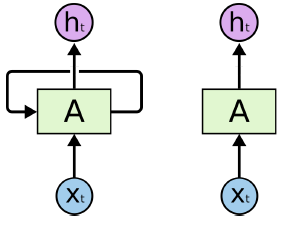
\includegraphics[width=0.5\textwidth]{figures/ml_theory/rnn_vs_ffnn_layer.png}
	\caption{Recurrent Layer (left) and Feed Forward Layer (right) illustration.}
	\label{fig:rnn_vs_ffnn}
\end{figure}

\subsubsection{Long Term Dependence Problem of Vanilla RNNs}
Conventional RNNs have problem with vanishing/exploding gradient problem. This causes long term dependence problem. For example, given word sequence, bold words in the following sentences are hard to predict with Vanilla RNN.

\centerline{The clouds are in the \textbf{sky}.}
\centerline{I grew up in France... I speak fluent \textbf{French}.}

In order to overcome this problem new architectures are developed such as Long Short Term Memory (LSTM) and Gated Recurrent Units (GRU).

\subsubsection{Long Short Term Memory}
LSTM is a special type of RNN. It is explicitly designed to allow learning long-term dependencies. A single LSTM cell has 4 neural layer while vanilla RNN layer has only one neural layer. In addition to hidden state $h_t$ , there is another state called cell state $C_t$. Information flow is controlled by 3 gates. 

\begin{figure}
	\centering
	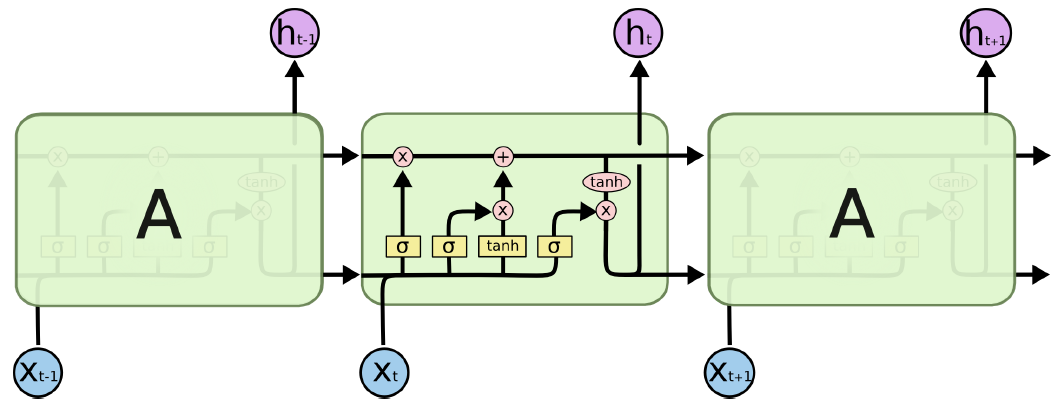
\includegraphics[width=0.95\textwidth]{figures/ml_theory/lstm/lstm_module.png}
	\caption{LSTM Cell.}
	\label{fig:lstm_cell}
\end{figure}

\textbf{Forget Gate}: Forget gate controls past memory. According to input, past memory is either kept or forgotten. Sigmoid function ($\sigma$) is used as activation function, applied elementwise.

\begin{equation}
\label{eqn:lstm_forget}
f_t = \sigma( [h_{t-1}; x_t] W_f + b_f) 
\end{equation}

\textbf{Input Gate}: Input gate controls contribution from input to cell state (memory). Hyperbolic tangent layer creates new candidate of cell state from input.

\begin{equation}
\label{eqn:lstm_inp}
i_t = \sigma( [h_{t-1}; x_t] W_i + b_{i}) 
\end{equation}

\begin{equation}
\label{eqn:lstm_cellstcand}
\hat{C}_t = \tanh( [h_{t-1}; x_t] W_C + b_C) 
\end{equation}

\textbf{Cell State Update}: Once what are to be forget and added are decided, cell state is updated.

\begin{equation}
\label{eqn:lstm_cellstupt}
C_t = f_t \odot C_{t-1} + i_t \odot \hat{C}_t
\end{equation}


\textbf{Output Gate}: Sigmoid layer decides what part of new cell state to be output. Cell state is filtered by tanh to push values to be in $(-1,1)$.

\begin{equation}
\label{eqn:lstm_out}
o_t = \sigma( [h_{t-1}; x_t] W_o + b_o) 
\end{equation}

\begin{equation}
h_t = o_t \odot \tanh(C_t)
\end{equation}

\subsection{Attention Mechanism}
As stated earlier, recurrent neural networks are prone to forget long term dependencies. LSTM and GRU are invented to overcome this problem. Although they reduced this problem, they cannot attend specific parts of the input. For example, for sentiment analysis, specific keywords are important to determine sentiment of a sentence. However, last state of encoded input is not able to remember that words. Therefore, people came with the idea of weighted avearing all states through time where weights depends on both input and output. 

Assume that input sequence $X \in \mathbb{R}^{T \times d_X}$ is encoded to $H \in \mathbb{R}^{T \times d_H}$. The context vector is calculated using weight vector $\alpha(t)$. 

Calculation of weight vector depends on the task. For each time step, a score function is calculated between hidden state $H \in \mathbb{R}^{T \times d_H}$ and query $\boldsymbol{q}$ (which may be many things depending on task). Also, score function is also depends on choice. Then, attention score is $\boldsymbol{\alpha} \in \mathbb{R}^{T}$ is calculated using arbitrary function $f$ depending on choice.

\begin{equation}
\begin{split}
\boldsymbol{\alpha} = & f(\boldsymbol{q}, H) \\
\mathrm{Attention}(q, H) = & \sum_{\tau=0}^{T} \alpha_{\tau} h_{\tau}
\end{split}
\end{equation}


\subsubsection{Transformer}
The Transformer was proposed in the paper Attention is All You Need \cite{vaswani_attention_2017} . Unlike recurrent networks, this architecture is solely builded on attention layers. 

A transformer layer consists of feed-forward and attention layers, which makes the mechanism special. Like RNNs, it can be used as both encoder and decoder. While encoder layers attend to itself, decoder layers attends both itself and encoded input.

\textbf{Attention Layer}: An attention layer is a mapping from 3 vectors called query $Q \in \mathbb{R}^{T \times d_k}$, key $K \in \mathbb{R}^{T \times d_k}$ and value $V \in \mathbb{R}^{T \times d_v}$ to output, where $T$ is time length, $d_k$ and $d_v$ are embedding dimensions. Output is weighted sum of values $V$ while weights are evaluated by compatibility metric of query $Q$ and key $K$. In vanilla transformer, compatibility of query and key is evaluated by dot product, normalizing by $sqrt(d_k)$. For a query, dot product with all keys are evaluated, then softmax function is applied to get weights of values. This approach is called Scaled Dot-product Attention.

\begin{equation}
\mathrm{Attention}(Q, K, V) = \mathrm{softmax}(\frac{Q^{T} K}{\sqrt{d_k}}) V
\end{equation}

\textbf{Multi-Head Attention}: Instead of performing single attention; keys, queries and values are linearly projected from $d_m$ dimensional vector space to $h$ different spaces using projection matrices. Then, attention is done $h$ times, and results are then concatenated and linearly projected to final values of the layer.

Projection matrices are model parameters, $W^Q_i \in \mathbb{R}^{d_m \times d_k}$, $W^K_i \in \mathbb{R}^{d_m \times d_k}$, $W^V_i \in \mathbb{R}^{d_m \times d_v}$ for $i=1,...,h$. Also output matrix is used to project multiple values into single one, $W^O \in \mathbb{R}^{h d_v \times d_m}$.

\begin{equation}
\begin{split}
\mathrm{MHA}(Q,K,V)= & \mathrm{Concat}(a_1, a_2, ... a_h)W^O \\
a_i = & \mathrm{Attention}(QW^Q_i,KW^K_i,VW^V_i)
\end{split}
\end{equation}

\textbf{Feed Forward Layer}: Both encoder and decoder contains feed forward layer, containing two linear transformations with ReLU activation.

\begin{equation}
\mathrm{FFN}(x) = \mathrm{ReLU}(xW_1+b)W_2+b_2
\end{equation}

\textbf{Layer Normalization}: Layer normalization is a layer to overcome xyz []. Given an input $x \in \mathbb{R}^K$, mean and variance statistics are evaluated along the dimensions \eqref{eq:layernorm_statistics}.

\begin{equation}
\label{eq:layernorm_statistics}
\begin{split}
\mu = & \frac{1}{K} \sum_{n=1}^{K} x_k \\
\sigma^2 = & \frac{1}{K} \sum_{n=1}^{K} (x_k-\mu)^2
\end{split}
\end{equation} 

Then, the input is first scaled to have zero mean and unity variance along dimensions. The term $\epsilon$ is added to prevent division by zero. Optionally, the result is scaled by elementwise multiplication by $\gamma \in \mathbb{R}^K$ and addition by $\beta \in \mathbb{R}^K$ where these are learnable parameters. 

\begin{equation}
\label{eqn:layernorm}
\mathrm{LN}(x) = \frac{x-\mu}{\sigma+\epsilon} * \gamma + \beta
\end{equation}

\textbf{Encoder Layer}: Encoder Layer starts with a residual self attention layer. Self attention means that query, key and value are same vectors. Then it is followed by feed forward neural layer, Both sublayers are employed with resudial connection with layer normalization, i.e summation of layer input and output is passed through layer normalization.

\begin{equation}
\begin{split}
att = & \mathrm{LN}(x+ \mathrm{MHA}(x,x,x)) \\
y = & \mathrm{LN}(att+ \mathrm{FFN}(att))
\end{split}
\end{equation}

\textbf{Decoder Layer}: Similar to encoder layer, decoder layer has also self-attention and feed forward layers. In addition, there is another attention layer which is over encoder outputs. Same as encoder, all sublayers have resudial connection with layer normalization. Let's call encoded sequence $e \in \mathbb{R}^{T \times d_m}$ and decoded sequence $d \in \mathbb{R}^{T \times d_m}$ (masked). Assume that the sequence decoded up to $t$th point in sequence. Then, $d_{t+1}$ is calculated as follows.

\begin{equation}
\begin{split}
att = & \mathrm{LN}(d_{1:t}+\mathrm{MHA}(d_{1:t},d_{1:t},d_{1:t})) \\
dec = & \mathrm{LN}(att+ \mathrm{MHA}(att,e,e)) \\
d_{t+1} = & \mathrm{LN}(dec+ \mathrm{FFN}(dec))
\end{split}
\end{equation}

\textbf{Positional encoding}: Since there are no recurrent or convolutional architecture in the model, sequential information needs to be embedded. Positional encodings has same dimension, so that input embeddings can be added to at the beginning of encoder or decoder stacks. For position $pos$, $2i$ or $2i+1$th dimension has following values ($i \in \mathbb{N}$), as proposed in the original paper.

\begin{equation}
\begin{split}
\mathrm{PE}_{pos,2i} = \sin(pos/10000^{2i/d_m}) \\
\mathrm{PE}_{pos,2i+1} = \cos(pos/10000^{2i/d_m})
\end{split}
\end{equation}

\subsubsection{Pre-Layer Normalized Transformer}
Original transformer architecture includes layer normalization operations after attention and feed-forward layers. It is unstable since gradients of output layers are high, so Pre-Layer Normalized transformer is proposed by \cite{xiong_layer_2020}. Moreover,  Parisotto et al. Xiong et al. \cite{parisotto_stabilizing_2019}. proposed gated transformer which also includes layer normalizations before attention and feedforward layer. They also stated that although gated architecture improves many RL tasks drastically, non-gated pre-layer normalized transformer are good enough. 

\begin{figure}
	\centering
	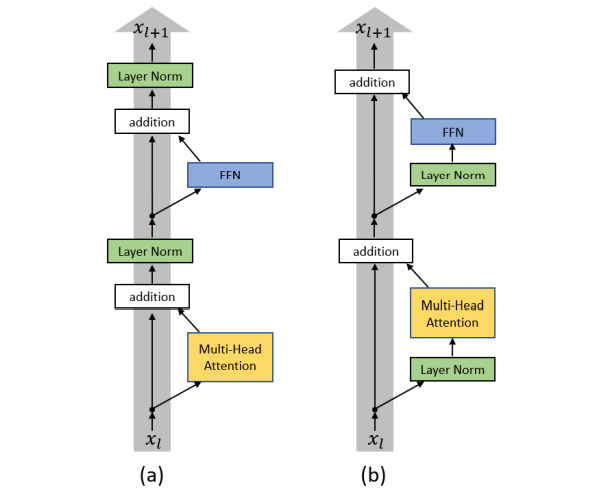
\includegraphics[width=0.95\textwidth]{figures/ml_theory/post_pre_trsf.png}
	\caption{(a) Post-LN Transformer layer, (b) Pre-LN Transformer
		layer.}
	\label{fig:post_pre_trsf}
\end{figure}

Encoder equations are as follows.

\begin{equation}
\begin{split}
att = & x+ \mathrm{MHA}(\mathrm{LN}(x),\mathrm{LN}(x),\mathrm{LN}(x)) \\
y = & att+ \mathrm{FFN}(\mathrm{LN}(att))
\end{split}
\end{equation}

Decoder equations are as follows.

\begin{equation}
\begin{split}
att = & d_{1:t}+\mathrm{MHA}(\mathrm{LN}(d_{1:t}),\mathrm{LN}(d_{1:t}),\mathrm{LN}(d_{1:t})) \\
dec = & att+ \mathrm{MHA}(\mathrm{LN}(att),\mathrm{LN}(att),\mathrm{LN}(att)) \\
d_{t+1} = & dec+ \mathrm{FFN}(\mathrm{LN}(dec))
\end{split}
\end{equation}

